\chapter{Definitions and Systems Overview}
\markboth{Definitions and Systems Overview}{}% To set left/right header
% \localtableofcontents

This chapter first introduce the notion of \emph{closed-loop sensitivity} that quantify how variations of some models parameters (supposed to be uncertain) affect the evolution of the system in closed-loop, i.e., by also taking into account any controller chosen for executing the task.
Then, it is presented how this sensitivity notion can be leveraged to derive \emph{uncertainty tubes} that bounds the system states evolution both in the \emph{input} and \emph{state} spaces.
Finally, the quadrotor robot and differential drive robot models used in this manuscript are introduced.

\section{Closed-loop sensitivity}
\subsection{Definition}

Consider an arbitrary dynamic system with a set of uncertain parameters $\p \in \mathbb{R}^{n_p}$ (i.e. model parameters that are difficult to evaluate or likely to vary during a motion).
The system dynamics can be described using the following set of ordinary differential equations (\myglsentry{odes}):
\begin{equation}\label{eq:dyna}
    \dot{\q}=\f(\q,\,\u,\,\p), \quad \q(t_0)=\q_{0},
\end{equation}
where $\q\in \mathbb{R}^{n_{q}}$ is the system state vector and $\u\in \mathbb{R}^{n_{u}}$ the control input vector.
Also, assume the presence of a controller $\boldmu$ of any form to track a \emph{desired trajectory} $\q_d(t)$ such that:
\begin{equation}\label{eq:ctrl}
     \left \{
     \begin{array}{l l}
          \dot{\bxi} = \g(\bxi,\,\q,\,\q_d,\,\p_n,\,\k_c,\,t), \quad \bxi(t_0)=\bxi_{0}, \\
          \u=\boldmu(\bxi,\,\q,\,\q_d,\,\p_n,\,\k_c,\,t), 
   \end{array} 
   \right .
\end{equation}
where $\bxi\in \mathbb{R}^{n_{\xi}}$ are the internal states of the controller (e.g., an integral action), $\k_{c}\in \mathbb{R}^{n_{k}}$ the controller gains, and $\p_{n}\in{\mathbb{R}^{n_{p}}}$ is the vector of "nominal" system parameters used in the control loop, i.e. the estimated nominal values of $\p$.

In line with the previous definitions, the following sections of this thesis will then differentiate between three types of state vectors of key importance:
\begin{enumerate}
  \item $\q_d$: The \emph{desired} system state vector which refers to the desired values of the controllable system states. This state vector is typically the output of a motion planner. Note that the dimension of this vector may differ from that of the real system because the vector represents a simplified or abstracted model, which might omit certain physical aspects or constraints that are present in the actual system, particularly in the case of under-actuated systems, where not all degrees of freedom are controlled.
  \item $\q_n$: The \emph{nominal} system state vector which represents the real state values of the system during the execution under nominal parameters (i.e. when the uncertain system parameters $\p$ perfectly match the parameter values used in the control loop $\p_n$). A distinction is made between the nominal states and the desired states, as they are generally not equal due to factors such as controller settings, transient behavior, etc.
  \item $\q$: The \emph{uncertain} system state vector which refers to the real state values of the system during the execution, influenced by a set of uncertain parameters.
\end{enumerate}
Note that the same notations apply to the control input vector as well (e.g., $\u_n$ represents the "nominal" control input values, i.e., when $\p=\p_n$).

It is possible to quantify how the presence of uncertain parameters (i.e. when the real system parameters $\p$ deviate from the nominal value $\p_n$ used in the control loop) affects the evolution of $\q(t)$ and $\u(t)$ according to the following matrices:
\begin{equation}\label{eq:sensi}
  \bPi(t)=\left.\frac{\partial \q(t)}{\partial \p}\right|_{\p=\p_n} \quad\quad \bTheta(t)=\left.\frac{\partial \u(t)}{\partial \p}\right|_{\p=\p_n}
\end{equation}
where $\bPi(t)\in \mathbb{R}^{n_q \times n_p}$ and $\bTheta(t)\in \mathbb{R}^{n_u \times n_p}$ are respectively defined in~\cite{cPi,cTh} as the \emph{state-sensitivity matrix} and the \emph{input-sensitivity matrix}.
A closed-form expression for Equation~(\ref{eq:sensi}) is, in general, not available. 
However, as shown in~\cite{cPi,cTh}, their evolution in time can be computed by differentiating Equation~(\ref{eq:sensi}) according to the following set of ODEs:
\begin{equation}\label{eq:dyna_sensi}
  \left \{
  \begin{array}{l l l}
       \dot{\bPi}(t) = \boldsymbol{\frac{\partial{f}}{\partial{q}}}\bPi+ \boldsymbol{\frac{\partial{f}}{\partial{u}}}\bTheta+ \boldsymbol{\frac{\partial{f}}{\partial{p}}}, \quad \bPi(t_0)=\bPi_0, \\
       \dot{\bPi}_{\xi}(t) = \boldsymbol{\frac{\partial{g}}{\partial{q}}}\bPi+ \boldsymbol{\frac{\partial{g}}{\partial{\xi}}}\bPi_{\xi}, \quad \bPi_{\xi}(t_0)=\bPi_{\xi0}, \\
       \bTheta(t) = \boldsymbol{\frac{\partial{h}}{\partial{q}}}\bPi+ \boldsymbol{\frac{\partial{h}}{\partial{\xi}}}\bPi_{\xi} 
  \end{array}
  \right .
\end{equation}
where $\bPixi(t)\in \mathbb{R}^{n_{\xi} \times n_p}$ represents the \emph{internal state sensitivity} matrix.

\subsection{Tube computation}

\begin{figure} [t]
  \centering
  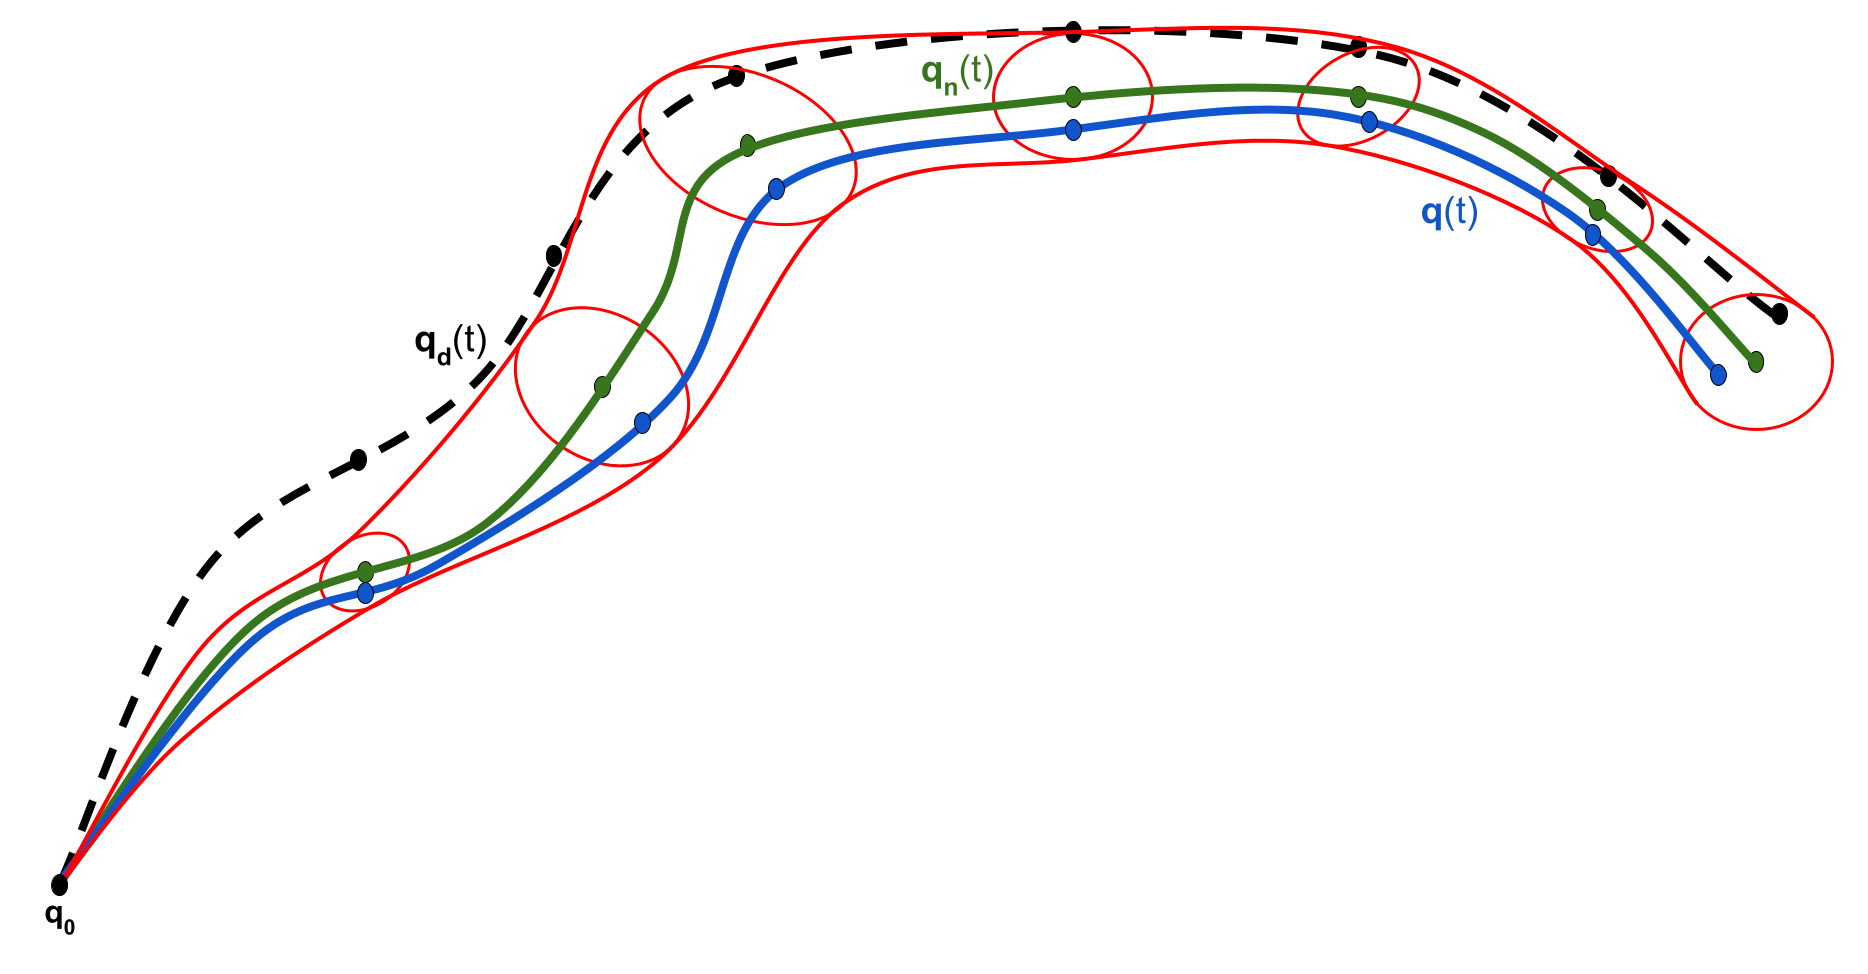
\includegraphics[width=0.8\linewidth]{figures/models/tubes.png} 
  \caption{Illustration of the uncertainty tube (red) and a perturbed trajectory $\q(t)$ (blue), centered around the nominal trajectory $\q_n(t)$ (green), which results from following the reference trajectory $\q_d(t)$ (dashed black).}%
  \label{fig:tubes}%
\end{figure}

\begin{figure} [t]
  \centering
  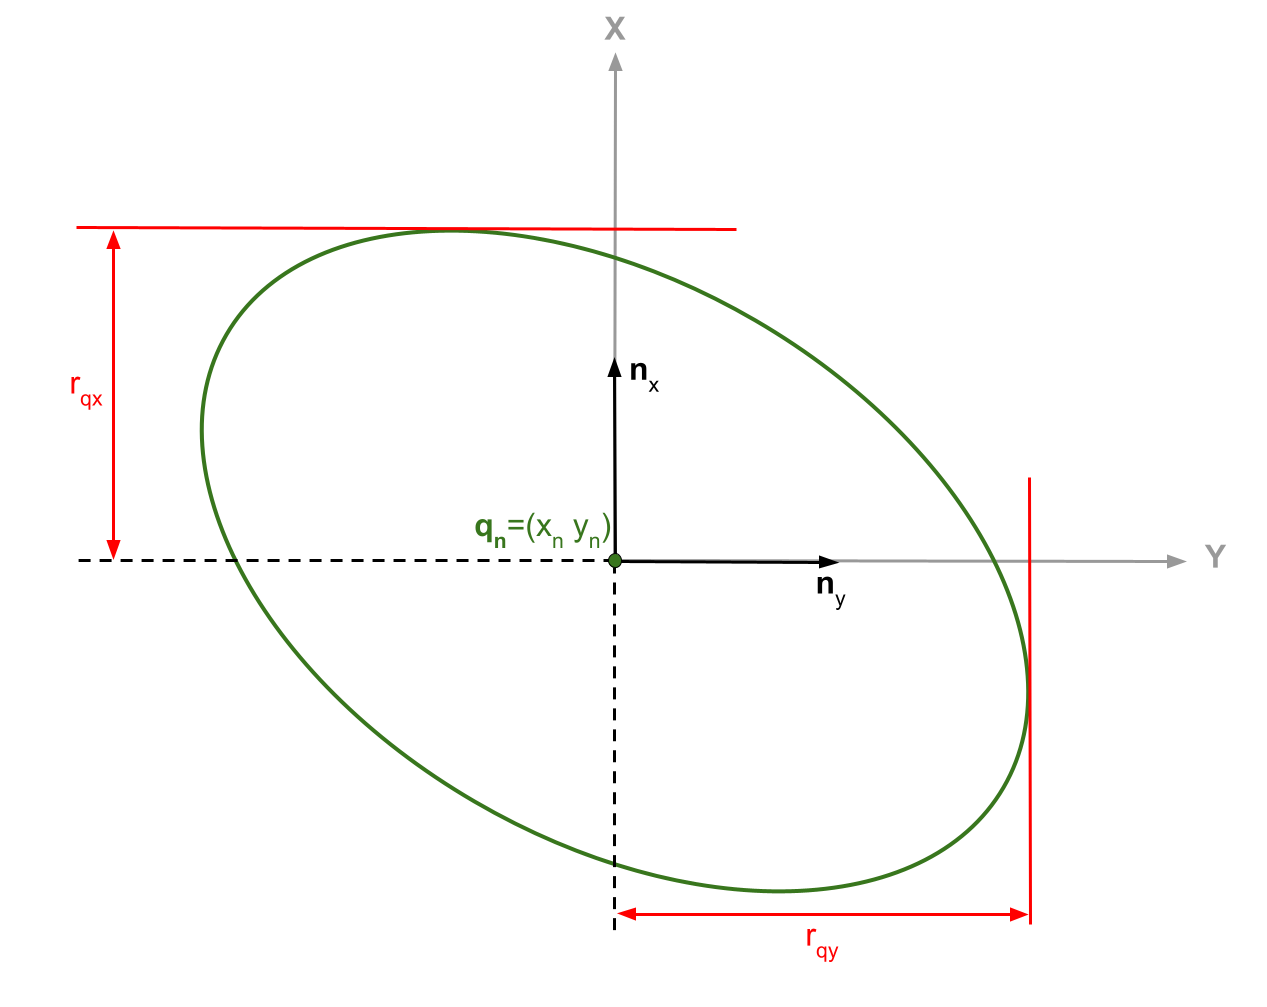
\includegraphics[width=0.8\linewidth]{figures/models/radius.png} 
  \caption{2D representation of an uncertainty ellipse (green) in the X-Y state space centered at $\q_n$, along with the tube radius (red) that illustrates the worst-case deviations along each canonical axis.}%
  \label{fig:ellips_radius}%
\end{figure}

A key feature of these matrices is their utility in deriving \emph{uncertainty tubes}, that bounds the closed-loop system trajectory $\q(t)$/$\u(t)$ around its nominal trajectory $\q_n(t)$/$\u_n(t)$ as shown in~\cite{cTube}.
The following remind how to establish such bounds around the nominal state trajectory $\q_n(t)$ by focusing solely on the state-sensitivity matrix $\bPi(t)$ for clarity. 
However, it is important to note that this same procedure can also be applied to compute bounds around the nominal input trajectory $\u_n(t)$ by leveraging the input-sensitivity matrix $\bTheta(t)$.

The uncertainty tube for each component of the state is characterized by a \emph{radius} which bounds the state component evolution from its nominal value over time, i.e. for the $i$-th component of the state ($q_i(t)$) the tube radius $r_{q,i}(t)$ is defined s.t.:
\begin{equation}\label{eq:bounds_q}
  q_{n,i}(t) - r_{q,i}(t) \leq q_i(t) \leq q_{n,i}(t) + r_{q,i}(t).
\end{equation}

Let $\Delta\q(t) = \q(t) - \q_n(t)$, representing the deviation of the perturbed trajectory from the nominal one, which we seek to bound.
Assume that for each uncertain parameter $p_{i \in [1, n_p]}$ in $\p$, we have a bounded parameter deviation $\delta p_i \in \mathbb{R}$ s.t. 
\begin{equation*}
  \forall i \in [1, n_p] ,p_i \in [p_{n_i}-\delta p_i, p_{n_i}+\delta p_i].
\end{equation*}
Such deviations can be mapped into the parameter space by mean of the following ellipsoid
\begin{equation}\label{eq:p_ellipsoid}
  \Delta\p^T \bW^{-1} \Delta\p \leq 1,
\end{equation}
where $\bW$ is the following diagonal weight matrix
\begin{equation*}
  \bW = \begin{bmatrix}
    \delta p_1^2 & 0 & \cdots & 0 \\
    0 & \delta p_2^2 & \cdots & 0 \\
    \vdots & \vdots & \ddots & \vdots \\
    0 & 0 & \cdots & \delta p_{n_p}^2
    \end{bmatrix} \in \mathbb{R}^{n_p \times n_p}.
\end{equation*}

Assuming small parameters variations (i.e. small $\delta \p$) it is possible to perform a first-order approximation around the nominal trajectory $\q_n(t)$ to obtain 
\begin{equation}\label{eq:approx}
  \Delta\q(t) =  \q(t) - \q_n(t) \approx \bPi(t) \Delta\p.
\end{equation}

Without loss of generality, for a well-chosen $\delta \p$ s.t. Equation~(\ref{eq:approx}) holds, ~\cite{cTube} has shown how to map the parameters ellipsoid from Equation~(\ref{eq:p_ellipsoid}) in the system state space in order to obtain the corresponding uncertainty ellipsoid
\begin{equation}\label{eq:q_ellipsoid}
  \Delta\q(t)^T (\bPi(t) \bW \bPi(t)^T)^\dag \Delta\q(t) \leq 1.
\end{equation}
However, it is important to note that the ellipsoid axes are in general not aligned with the canonical basis of the state space.

Nevertheless, it has been shown in ~\cite{cTube} how to obtain the tube radius along the $i$-th component of the state $q_i(t)$ by mean of the following projection:
\begin{equation}\label{eq:radius}
  r_{q,i}(t) =  \sqrt{\boldsymbol{n_i}^{T} \boldsymbol{K_{\Pi}}(t) \boldsymbol{n_i}},
\end{equation}
where $\boldsymbol{n}_i$ is the unit-norm vector of the $i$-th state space component, and $\boldsymbol{K_{\Pi}}(t) = \boldsymbol{\Pi}(t)\boldsymbol{W}\boldsymbol{\Pi}(t)^T$ is the kernel matrix of Equation~(\ref{eq:q_ellipsoid}).
It is important to note that the radius along the $i$-th component represents the maximum possible deviation in that direction and does not directly correspond to the semi-axes of the uncertainty ellipsoid as depicted in Figure~\ref{fig:ellips_radius}.

Finally, it is important to remind that since the uncertainty tube radii depend on the state sensitivity $\boldsymbol{\Pi}(t)$, it is necessary to solve the set of ODEs represented by Equation~(\ref{eq:dyna}), Equation~(\ref{eq:ctrl}), and Equation~(\ref{eq:dyna_sensi}) beforehand.
Additionally, note how, in general, the tube radius does not necessarily increase monotonically due to the influence of feedback action as illustrated in Figure~\ref{fig:tubes}, despite the cumulative effect of uncertainties over time. 

\section{Models considered in this thesis}

To offer a general approach applicable to various robots and controllers, this thesis considers a quadrotor and a differential drive robot, along with two distinct controllers and interpolation methods, which are detailed in the following sections.

\subsection{Quadrotor robot} \label{sec:quad_model}

\subsubsection{Dynamic model}

\begin{figure} [t]
    \centering
    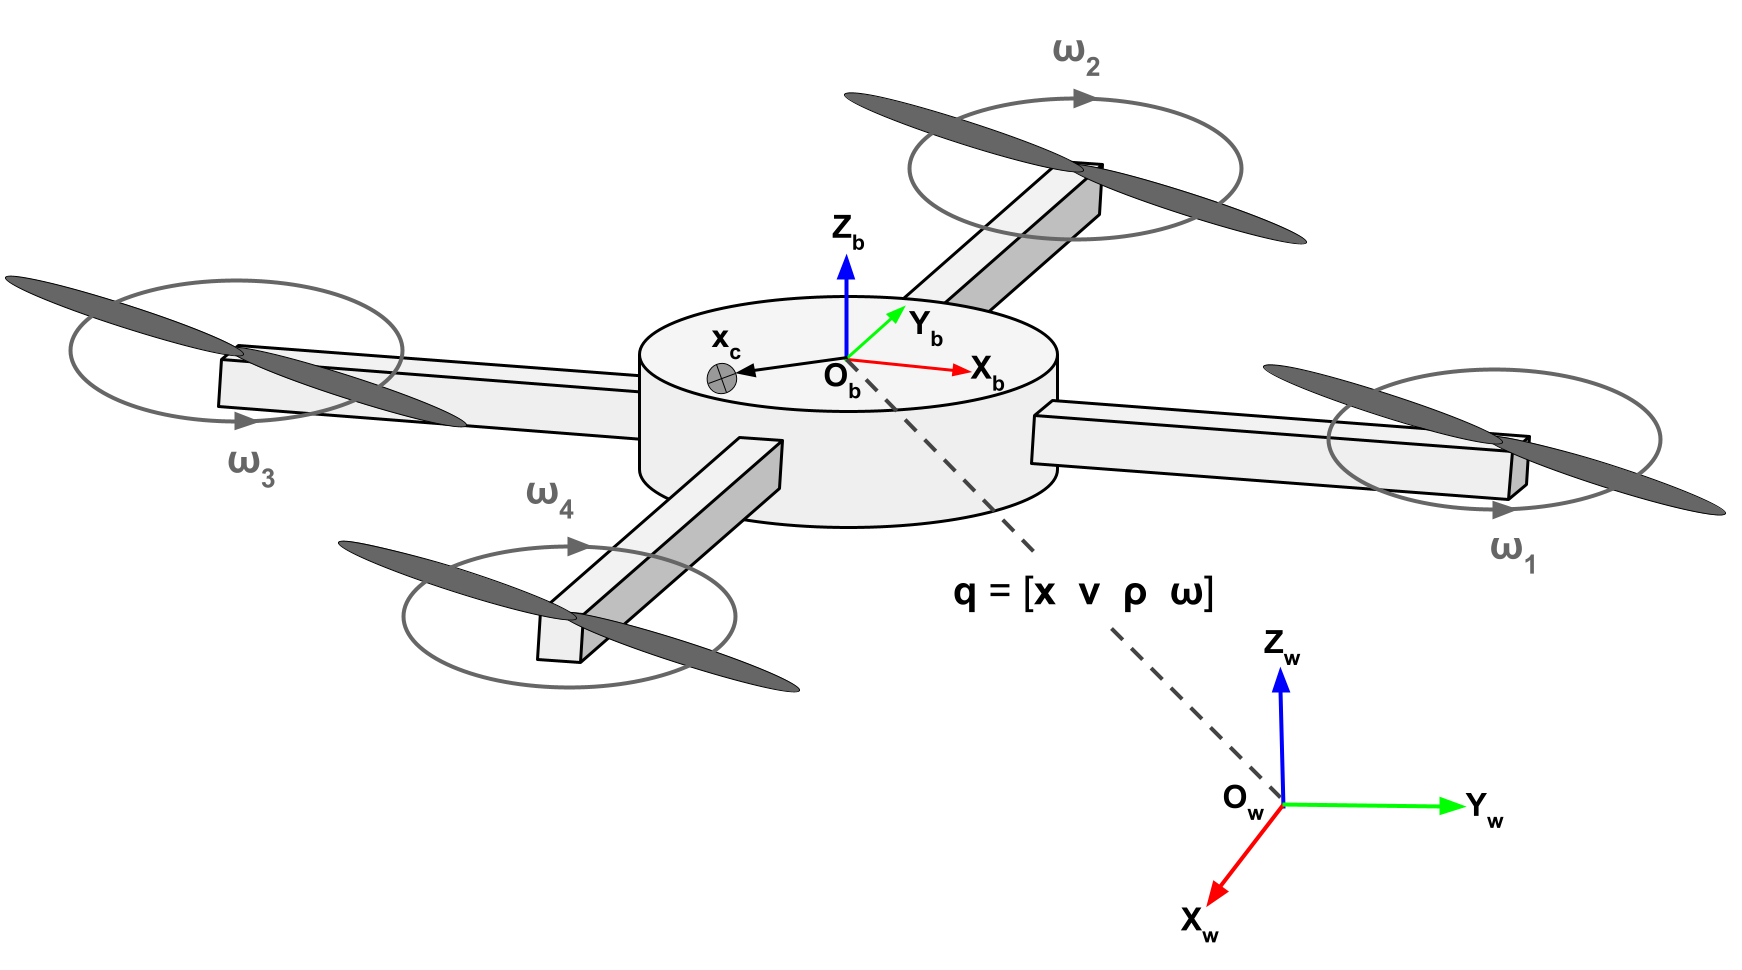
\includegraphics[width=0.8\linewidth]{figures/models/drone.png} 
    \caption{Quadrotor robot representation with a shift in the center of mass.}%
    \label{fig:quad}%
\end{figure}

Let the ENU (East North Up) world frame be defined as $F_W \allowbreak = \allowbreak \{O_W, \allowbreak X_W, \allowbreak Y_W, \allowbreak Z_W\}$ and $F_B = \allowbreak\{O_B, \allowbreak X_B, \allowbreak Y_B, \allowbreak Z_B\}$ be the quadrotor body frame attached to its geometric center ($O_B$).
The state of the quadrotor is defined as $\boldsymbol{q} = [\boldsymbol{x}  \, \boldsymbol{v} \, \boldsymbol{\rho} \, \boldsymbol{\omega}]$ where $\boldsymbol{x} = [x \, y \,z] \in \mathbb{R}^{3}$ and $\boldsymbol{v} = [v_x \, v_y \,v_z] \in \mathbb{R}^{3}$ are respectively the position and velocity vector of $O_B$ expressed in $F_W$. The body orientation w.r.t. $F_W$ is represented by the unitary quaternion  $\boldsymbol{\rho}$ and its angular velocity as $\boldsymbol{\omega} = [\omega_x \, \omega_y \, \omega_z] \in \mathbb{R}^{3}$. 
Finally, let $\boldsymbol{R(\rho)}$ be the rotation matrix associated to $\boldsymbol{\rho}$.

We consider that the center of mass (\myglsentry{com}) is displaced from the robot geometric center of an offset $\boldsymbol{x_{c}} = [x_{cx}, x_{cy}, x_{cz}]$ expressed in $F_B$ as depicted in Figure.~\ref{fig:quad}. 
This displacement can occur due to onboard sensors, the presence of a payload, or other factors.
Under this consideration, the total force ($\boldsymbol{f_{tot}}$) and torque ($\boldsymbol{\tau_{tot}}$) acting on the quadrotor can be expressed by taking an additional fictitious force due to the displaced CoM in $F_B$ s.t. 
\[
    \begin{array}{@{}l@{}l@{}}
        \boldsymbol{f_{tot}} &= f Z_W - mg\boldsymbol{R(\rho)}^TZ_W-m[\boldsymbol{\omega}]_{\times}[\boldsymbol{\omega}]_{\times}\boldsymbol{x_c} 
          
          \\
      
       \boldsymbol{\tau_{tot}} &= \boldsymbol{\tau}-mg[\boldsymbol{x_c}]_{\times}\boldsymbol{R(\rho)}^{T}Z_W - [\boldsymbol{\omega}]_{\times}\boldsymbol{J}\boldsymbol{\omega}
  \end{array}
\]
where $f$ and $\boldsymbol{\tau}$ are the propeller total thrust and torques, $m$ is the mass and $\boldsymbol{J}$ is the inertia matrix of the system. 
By considering the spatial inertia matrix
\[
\boldsymbol{S} =   \left( {\begin{array}{cc}
    m\boldsymbol{I_3} & -m[\boldsymbol{x_c}]_{\times} \\
    m[\boldsymbol{x_c}]_{\times} & \boldsymbol{J} \\
  \end{array} } \right)
\]
one finally gets the body frame linear acceleration $\boldsymbol{\alpha}$ and angular acceleration $\boldsymbol{\eta}$
as: 
$
\left( 
    \boldsymbol{\alpha}^T \; \boldsymbol{\eta}^T \right)^T 
  =
  \boldsymbol{S}^{-1}
  \left( \boldsymbol{f_{tot}}^T \;
    \boldsymbol{\tau_{tot}}^T \right)^T. 
$
The dynamic model is then defined as follows:
\begin{equation}\label{eq:dynamic}
    \Dot{\q}
    =
     \left \{
     \begin{array}{l l}
           \dot{\boldsymbol{x}} = \boldsymbol{v} \\
           
           \dot{\boldsymbol{v}}= \boldsymbol{\alpha} \\

           \dot{\boldsymbol{\rho}}=\frac{1}{2}
               \boldsymbol{\rho} \otimes \begin{bmatrix}
                                          0 \\
                                          \boldsymbol{\omega}
                                          \end{bmatrix} \\
           
           \dot{\boldsymbol{\omega}}=\boldsymbol{\eta}
   \end{array}
   \right .
\end{equation}

As tracking controller, we consider the so-called Lee (or geometric) controller~\cite{cLee} where the control inputs are the squared rotor speeds $\u = [\omega_{1}^2 \, \omega_{2}^2 \, \omega_{3}^2 \, \omega_{4}^2]^T$ that are related to $f$ and $\boldsymbol{\tau}$ by mean of a standard allocation matrix $\boldsymbol{T}$ s.t.
\begin{equation}
  \begin{bmatrix}
    f \\
    \boldsymbol{\tau}
    \end{bmatrix} = \boldsymbol{T}(l, k_f, k_{\tau}) \u,
\end{equation}
where $k_f$ and $k_{\tau}$ refer to the thrust and drag coefficients of the propellers respectively, and $l$ stands for the quadrotor arms length.

The uncertain parameters vector is defined as
$\p$ = $[m, \, x_{cx}, \, x_{cy}, \, J_{x}, \, J_{y}, \,J_{z}]^T \in \mathbb{R}^{6}$, which represents parameters that are difficult to evaluate or likely to vary during execution. 
We chose as nominal parameters $\p_{c}$ = $[1.113, 0.0, 0.0, 0.015, 0.015, 0.007]^T$ and their associated uncertainty range $\delta\p = [7\%, 3cm, 3cm, 10\%, 10\%, 10\%]^T$, which represents the percentage variation of the parameters w.r.t. their associated nominal value, except for $x_{cx}$ and $x_{cy}$ whose nominal values are zeros.

\subsubsection{State interpolation}

\subsection{Differential drive robot}

\subsubsection{Dynamic model}
\subsubsection{State interpolation}

\todomarker{}